\documentclass[border=8pt,tikz]{standalone}
\usepackage{fontspec}
\usepackage{babel}
\babelprovide[import, main]{vietnamese}
\babelfont{rm}{Latin Modern Roman}
\babelfont{sf}{Latin Modern Roman}
\babelfont{tt}{Latin Modern Roman}
\usepackage{tikz}
\usetikzlibrary{arrows.meta,calc,positioning,backgrounds}

\definecolor{navy}{HTML}{0F2C59}
\definecolor{deepblue}{HTML}{1D4ED8}
\definecolor{teal}{HTML}{0D9488}
\definecolor{darkteal}{HTML}{0F766E}
\definecolor{crimson}{HTML}{DC2626}
\definecolor{amber}{HTML}{D97706}
\definecolor{gold}{HTML}{F59E0B}
\definecolor{purple}{HTML}{6D28D9}
\definecolor{slate}{HTML}{334155}
\definecolor{lightgray}{HTML}{F8FAFC}

\begin{document}
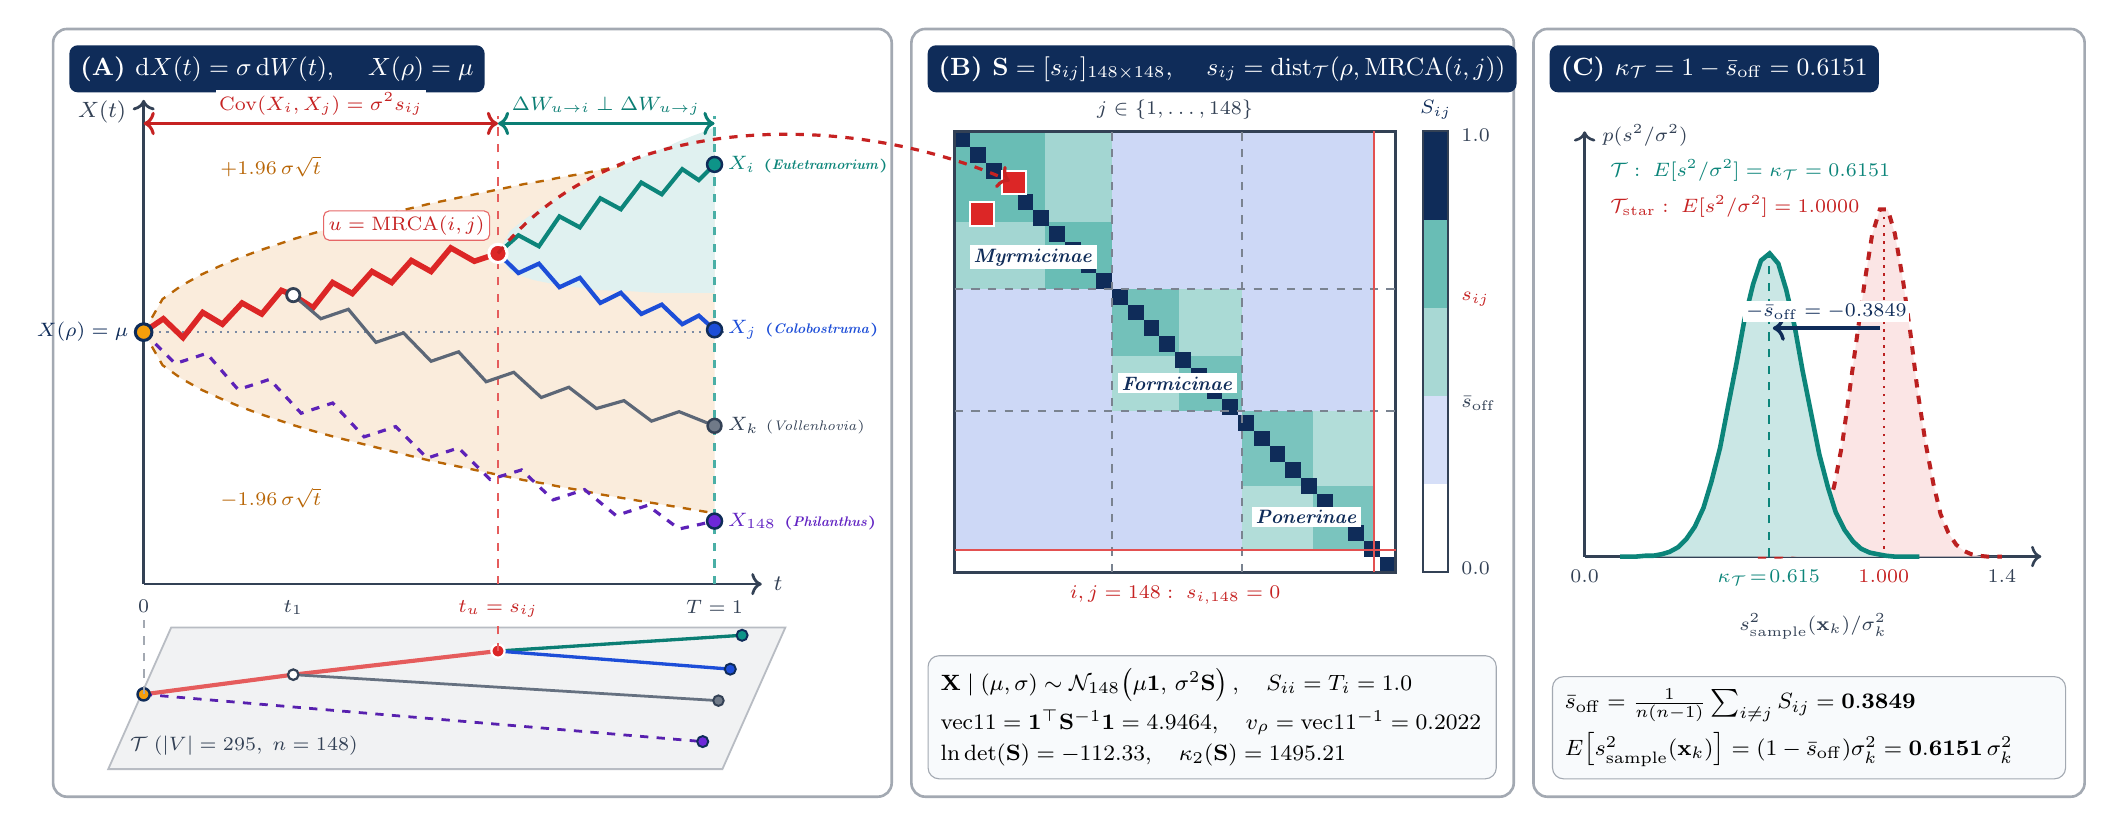
\begin{tikzpicture}

% ==============================================================================
% PANEL (A): 3D BM SDE TRAJECTORIES & MRCA(i,j)
% ==============================================================================
\filldraw[fill=white, draw=slate!45, line width=0.95pt, rounded corners=5pt] (0.00,0.00) rectangle (10.65,9.75);
\node[fill=navy, text=white, rounded corners=3pt, inner sep=4pt, anchor=north west, font=\small\bfseries]
    at (0.20,9.55) {(A) $\mathrm{d}X(t) = \sigma\,\mathrm{d}W(t),\quad X(\rho) = \mu$};

% Base phylogenetic plane
\filldraw[fill=slate!7, draw=slate!35, line width=0.65pt]
    (0.70,0.35) -- (8.50,0.35) -- (9.30,2.15) -- (1.50,2.15) -- cycle;
\node[text=slate, anchor=south west, font=\scriptsize\bfseries] at (0.85,0.40) {$\mathcal{T}\; (|V|=295,\; n=148)$};

\draw[draw=crimson!75, line width=1.5pt] (1.15,1.30) -- (3.05,1.55) -- (5.65,1.85);
\draw[draw=teal!85!black, line width=1.2pt] (5.65,1.85) -- (8.75,2.05);
\draw[draw=deepblue, line width=1.2pt] (5.65,1.85) -- (8.60,1.62);
\draw[draw=slate!75, line width=1.0pt] (3.05,1.55) -- (8.45,1.22);
\draw[draw=purple!80!black, line width=1.0pt, dashed] (1.15,1.30) -- (8.25,0.70);

\filldraw[fill=gold, draw=navy, line width=0.9pt] (1.15,1.30) circle (2.2pt);
\filldraw[fill=white, draw=slate, line width=0.8pt] (3.05,1.55) circle (1.9pt);
\filldraw[fill=crimson, draw=white, line width=0.8pt] (5.65,1.85) circle (2.4pt);
\filldraw[fill=teal, draw=navy, line width=0.7pt] (8.75,2.05) circle (2.0pt);
\filldraw[fill=deepblue, draw=navy, line width=0.7pt] (8.60,1.62) circle (2.0pt);
\filldraw[fill=slate!70, draw=slate, line width=0.7pt] (8.45,1.22) circle (1.9pt);
\filldraw[fill=purple, draw=navy, line width=0.7pt] (8.25,0.70) circle (2.0pt);

% 95% Gaussian Diffusion Envelopes
\fill[fill=amber!14] (1.15,5.90) -- (1.39,6.32) -- (1.63,6.49) -- (1.88,6.63) -- (2.12,6.74) -- (2.36,6.84) -- (2.60,6.93) -- (2.84,7.01) -- (3.08,7.09) -- (3.32,7.16) -- (3.57,7.23) -- (3.81,7.29) -- (4.05,7.35) -- (4.29,7.41) -- (4.53,7.47) -- (4.78,7.53) -- (5.02,7.58) -- (5.26,7.63) -- (5.50,7.68) -- (5.74,7.73) -- (5.98,7.78) -- (6.22,7.82) -- (6.47,7.87) -- (6.71,7.91) -- (6.95,7.96) -- (7.19,8.00) -- (7.43,8.04) -- (7.68,8.08) -- (7.92,8.12) -- (8.16,8.16) -- (8.40,8.20) -- (8.40,3.60) -- (8.16,3.64) -- (7.92,3.68) -- (7.68,3.72) -- (7.43,3.76) -- (7.19,3.80) -- (6.95,3.84) -- (6.71,3.89) -- (6.47,3.93) -- (6.22,3.98) -- (5.98,4.02) -- (5.74,4.07) -- (5.50,4.12) -- (5.26,4.17) -- (5.02,4.22) -- (4.78,4.27) -- (4.53,4.33) -- (4.29,4.39) -- (4.05,4.45) -- (3.81,4.51) -- (3.57,4.57) -- (3.32,4.64) -- (3.08,4.71) -- (2.84,4.79) -- (2.60,4.87) -- (2.36,4.96) -- (2.12,5.06) -- (1.88,5.17) -- (1.63,5.31) -- (1.39,5.48) -- (1.15,5.90) -- cycle;
\draw[draw=amber!85!black, line width=0.85pt, dashed] (1.15,5.90) -- (1.39,6.32) -- (1.63,6.49) -- (1.88,6.63) -- (2.12,6.74) -- (2.36,6.84) -- (2.60,6.93) -- (2.84,7.01) -- (3.08,7.09) -- (3.32,7.16) -- (3.57,7.23) -- (3.81,7.29) -- (4.05,7.35) -- (4.29,7.41) -- (4.53,7.47) -- (4.78,7.53) -- (5.02,7.58) -- (5.26,7.63) -- (5.50,7.68) -- (5.74,7.73) -- (5.98,7.78) -- (6.22,7.82) -- (6.47,7.87) -- (6.71,7.91) -- (6.95,7.96) -- (7.19,8.00) -- (7.43,8.04) -- (7.68,8.08) -- (7.92,8.12) -- (8.16,8.16) -- (8.40,8.20);
\draw[draw=amber!85!black, line width=0.85pt, dashed] (1.15,5.90) -- (1.39,5.48) -- (1.63,5.31) -- (1.88,5.17) -- (2.12,5.06) -- (2.36,4.96) -- (2.60,4.87) -- (2.84,4.79) -- (3.08,4.71) -- (3.32,4.64) -- (3.57,4.57) -- (3.81,4.51) -- (4.05,4.45) -- (4.29,4.39) -- (4.53,4.33) -- (4.78,4.27) -- (5.02,4.22) -- (5.26,4.17) -- (5.50,4.12) -- (5.74,4.07) -- (5.98,4.02) -- (6.22,3.98) -- (6.47,3.93) -- (6.71,3.89) -- (6.95,3.84) -- (7.19,3.80) -- (7.43,3.76) -- (7.68,3.72) -- (7.92,3.68) -- (8.16,3.64) -- (8.40,3.60);
\fill[fill=teal!13] (5.65,6.90) -- (5.80,7.18) -- (5.96,7.31) -- (6.11,7.42) -- (6.26,7.52) -- (6.41,7.61) -- (6.57,7.69) -- (6.72,7.77) -- (6.87,7.84) -- (7.03,7.92) -- (7.18,7.99) -- (7.33,8.06) -- (7.48,8.12) -- (7.64,8.19) -- (7.79,8.25) -- (7.94,8.32) -- (8.09,8.38) -- (8.25,8.44) -- (8.40,8.50) -- (8.40,6.40) -- (8.25,6.40) -- (8.09,6.40) -- (7.94,6.40) -- (7.79,6.40) -- (7.64,6.40) -- (7.48,6.41) -- (7.33,6.42) -- (7.18,6.42) -- (7.03,6.43) -- (6.87,6.44) -- (6.72,6.46) -- (6.57,6.48) -- (6.41,6.50) -- (6.26,6.53) -- (6.11,6.56) -- (5.96,6.61) -- (5.80,6.68) -- (5.65,6.90) -- cycle;

\node[text=amber!85!black, anchor=south west, font=\scriptsize\bfseries] at (2.00,7.75) {$+1.96\,\sigma\sqrt{t}$};
\node[text=amber!85!black, anchor=north west, font=\scriptsize\bfseries] at (2.00,4.05) {$-1.96\,\sigma\sqrt{t}$};

% Axes & Time Slices
\draw[->, draw=slate, line width=1.0pt] (1.15,2.70) -- (9.00,2.70);
\draw[->, draw=slate, line width=1.0pt] (1.15,2.70) -- (1.15,8.85);
\node[text=slate, anchor=west, font=\footnotesize\bfseries] at (9.03,2.70) {$t$};
\node[text=slate, anchor=east, font=\footnotesize\bfseries] at (1.05,8.70) {$X(t)$};

\draw[draw=slate!45, line width=0.65pt, dashed] (1.15,1.30) -- (1.15,2.25);
\draw[draw=crimson!75, line width=0.95pt, dashed] (5.65,1.85) -- (5.65,2.25);
\draw[draw=crimson!75, line width=0.95pt, dashed] (5.65,2.70) -- (5.65,8.65);
\draw[draw=teal!75, line width=0.75pt, dashed] (8.40,2.70) -- (8.40,8.65);
\draw[draw=navy!55, line width=0.75pt, dotted] (1.15,5.90) -- (8.55,5.90);

\node[text=slate, anchor=north, font=\scriptsize] at (1.15,2.62) {$0$};
\node[text=slate, anchor=north, font=\scriptsize] at (3.05,2.62) {$t_1$};
\node[text=crimson!90!black, anchor=north, font=\scriptsize\bfseries] at (5.65,2.62) {$t_u = s_{ij}$};
\node[text=slate, anchor=north, font=\scriptsize] at (8.40,2.62) {$T = 1$};
\node[text=navy, anchor=east, font=\scriptsize\bfseries] at (1.08,5.90) {$X(\rho)=\mu$};

% Sample Paths X(t)
\draw[draw=crimson, line width=2.0pt]
    (1.15,5.90) -- (1.40,6.07) -- (1.65,5.83) -- (1.90,6.15) -- (2.15,6.00)
    -- (2.40,6.27) -- (2.65,6.13) -- (2.90,6.43) -- (3.05,6.37)
    -- (3.30,6.21) -- (3.55,6.53) -- (3.80,6.39) -- (4.05,6.67)
    -- (4.30,6.53) -- (4.55,6.81) -- (4.80,6.67) -- (5.05,6.97)
    -- (5.35,6.80) -- (5.65,6.90);

\draw[draw=teal!90!black, line width=1.5pt]
    (5.65,6.90) -- (5.91,7.13) -- (6.17,6.99) -- (6.43,7.37) -- (6.69,7.23)
    -- (6.95,7.60) -- (7.21,7.46) -- (7.47,7.80) -- (7.73,7.65)
    -- (7.99,7.97) -- (8.20,7.83) -- (8.40,8.03);

\draw[draw=deepblue, line width=1.5pt]
    (5.65,6.90) -- (5.91,6.65) -- (6.17,6.77) -- (6.43,6.47) -- (6.69,6.59)
    -- (6.95,6.27) -- (7.21,6.40) -- (7.47,6.13) -- (7.73,6.25)
    -- (7.99,6.00) -- (8.20,6.11) -- (8.40,5.93);

\draw[draw=slate!80, line width=1.15pt]
    (3.05,6.37) -- (3.40,6.07) -- (3.75,6.19) -- (4.10,5.77) -- (4.45,5.89)
    -- (4.80,5.53) -- (5.15,5.65) -- (5.50,5.27) -- (5.85,5.39)
    -- (6.20,5.07) -- (6.55,5.20) -- (6.90,4.93) -- (7.25,5.03)
    -- (7.60,4.77) -- (7.95,4.89) -- (8.40,4.71);

\draw[draw=purple!85!black, line width=1.15pt, dashed]
    (1.15,5.90) -- (1.55,5.50) -- (1.95,5.63) -- (2.35,5.17) -- (2.75,5.30)
    -- (3.15,4.87) -- (3.55,5.00) -- (3.95,4.57) -- (4.35,4.70)
    -- (4.75,4.30) -- (5.15,4.43) -- (5.55,4.03) -- (5.95,4.15)
    -- (6.35,3.77) -- (6.75,3.90) -- (7.15,3.57) -- (7.55,3.70)
    -- (7.95,3.40) -- (8.40,3.50);

\filldraw[fill=gold, draw=navy, line width=1.1pt] (1.15,5.90) circle (3.0pt);
\filldraw[fill=white, draw=slate, line width=1.0pt] (3.05,6.37) circle (2.4pt);
\filldraw[fill=crimson, draw=white, line width=1.1pt] (5.65,6.90) circle (3.3pt);
\filldraw[fill=teal, draw=navy, line width=0.9pt] (8.40,8.03) circle (2.7pt);
\filldraw[fill=deepblue, draw=navy, line width=0.9pt] (8.40,5.93) circle (2.7pt);
\filldraw[fill=slate!70, draw=slate, line width=0.9pt] (8.40,4.71) circle (2.5pt);
\filldraw[fill=purple, draw=navy, line width=0.9pt] (8.40,3.50) circle (2.7pt);

% Compact symbol-only labels at leaves and MRCA
\node[text=teal!90!black, anchor=west, font=\scriptsize\bfseries] at (8.45,8.03) {$X_i$ {\tiny(\textit{Eutetramorium})}};
\node[text=deepblue, anchor=west, font=\scriptsize\bfseries] at (8.45,5.93) {$X_j$ {\tiny(\textit{Colobostruma})}};
\node[text=slate, anchor=west, font=\scriptsize] at (8.45,4.71) {$X_k$ {\tiny(\textit{Vollenhovia})}};
\node[text=purple!90!black, anchor=west, font=\scriptsize\bfseries] at (8.45,3.50) {$X_{148}$ {\tiny(\textit{Philanthus})}};

\node[fill=white, draw=crimson!70, rounded corners=2pt, inner sep=1.8pt, text=crimson!90!black, anchor=south east, font=\scriptsize\bfseries]
    at (5.55,7.06) {$u = \mathrm{MRCA}(i,j)$};

\draw[<->, draw=crimson!90!black, line width=1.1pt] (1.15,8.55) -- (5.65,8.55);
\node[fill=white, inner sep=1.2pt, text=crimson!90!black, anchor=south, font=\scriptsize\bfseries]
    at (3.40,8.60) {$\mathrm{Cov}(X_i,X_j) = \sigma^2 s_{ij}$};

\draw[<->, draw=teal!85!black, line width=1.1pt] (5.65,8.55) -- (8.40,8.55);
\node[fill=white, inner sep=1.2pt, text=teal!85!black, anchor=south, font=\scriptsize\bfseries]
    at (7.02,8.60) {$\Delta W_{u\to i} \perp \Delta W_{u\to j}$};

% ==============================================================================
% PANEL (B): COVARIANCE MATRIX S = [s_ij]_{148 x 148}
% ==============================================================================
\filldraw[fill=white, draw=slate!45, line width=0.95pt, rounded corners=5pt] (10.90,0.00) rectangle (18.55,9.75);
\node[fill=navy, text=white, rounded corners=3pt, inner sep=4pt, anchor=north west, font=\small\bfseries]
    at (11.10,9.55) {(B) $\mathbf{S} = [s_{ij}]_{148 \times 148},\quad s_{ij} = \mathrm{dist}_{\mathcal{T}}(\rho, \mathrm{MRCA}(i,j))$};

% Heatmap at (11.45, 2.85) of size 5.60 x 5.60 cm
\fill[fill=deepblue!10] (11.45,2.85) rectangle (17.05,8.45);
\fill[fill=white] (11.45,2.85) rectangle (17.05,3.13);
\fill[fill=white] (16.77,2.85) rectangle (17.05,8.45);
\fill[fill=deepblue!22] (11.45,3.13) rectangle (16.77,8.45);

% Clade 1: Myrmicinae
\fill[fill=teal!38] (11.45,6.45) rectangle (13.45,8.45);
\fill[fill=teal!62] (11.45,7.30) rectangle (12.60,8.45);
\fill[fill=teal!62] (12.60,6.45) rectangle (13.45,7.30);

% Clade 2: Formicinae
\fill[fill=teal!35] (13.45,4.90) rectangle (15.10,6.45);
\fill[fill=teal!58] (13.45,5.60) rectangle (14.30,6.45);
\fill[fill=teal!58] (14.30,4.90) rectangle (15.10,5.60);

% Clade 3: Ponerinae
\fill[fill=teal!32] (15.10,3.13) rectangle (16.77,4.90);
\fill[fill=teal!55] (15.10,3.95) rectangle (16.00,4.90);
\fill[fill=teal!55] (16.00,3.13) rectangle (16.77,3.95);

\fill[fill=navy] (11.45,8.25) rectangle (11.65,8.45);
\fill[fill=navy] (11.65,8.05) rectangle (11.85,8.25);
\fill[fill=navy] (11.85,7.85) rectangle (12.05,8.05);
\fill[fill=navy] (12.05,7.65) rectangle (12.25,7.85);
\fill[fill=navy] (12.25,7.45) rectangle (12.45,7.65);
\fill[fill=navy] (12.45,7.25) rectangle (12.65,7.45);
\fill[fill=navy] (12.65,7.05) rectangle (12.85,7.25);
\fill[fill=navy] (12.85,6.85) rectangle (13.05,7.05);
\fill[fill=navy] (13.05,6.65) rectangle (13.25,6.85);
\fill[fill=navy] (13.25,6.45) rectangle (13.45,6.65);
\fill[fill=navy] (13.45,6.25) rectangle (13.65,6.45);
\fill[fill=navy] (13.65,6.05) rectangle (13.85,6.25);
\fill[fill=navy] (13.85,5.85) rectangle (14.05,6.05);
\fill[fill=navy] (14.05,5.65) rectangle (14.25,5.85);
\fill[fill=navy] (14.25,5.45) rectangle (14.45,5.65);
\fill[fill=navy] (14.45,5.25) rectangle (14.65,5.45);
\fill[fill=navy] (14.65,5.05) rectangle (14.85,5.25);
\fill[fill=navy] (14.85,4.85) rectangle (15.05,5.05);
\fill[fill=navy] (15.05,4.65) rectangle (15.25,4.85);
\fill[fill=navy] (15.25,4.45) rectangle (15.45,4.65);
\fill[fill=navy] (15.45,4.25) rectangle (15.65,4.45);
\fill[fill=navy] (15.65,4.05) rectangle (15.85,4.25);
\fill[fill=navy] (15.85,3.85) rectangle (16.05,4.05);
\fill[fill=navy] (16.05,3.65) rectangle (16.25,3.85);
\fill[fill=navy] (16.25,3.45) rectangle (16.45,3.65);
\fill[fill=navy] (16.45,3.25) rectangle (16.65,3.45);
\fill[fill=navy] (16.65,3.05) rectangle (16.85,3.25);
\fill[fill=navy] (16.85,2.85) rectangle (17.05,3.05);

\filldraw[fill=crimson, draw=white, line width=0.7pt] (12.05,7.65) rectangle (12.35,7.95);
\filldraw[fill=crimson, draw=white, line width=0.7pt] (11.65,7.25) rectangle (11.95,7.55);

\draw[draw=slate, line width=0.9pt] (11.45,2.85) rectangle (17.05,8.45);
\draw[draw=slate!65, line width=0.55pt, dashed] (13.45,2.85) -- (13.45,8.45);
\draw[draw=slate!65, line width=0.55pt, dashed] (11.45,6.45) -- (17.05,6.45);
\draw[draw=slate!65, line width=0.55pt, dashed] (15.10,2.85) -- (15.10,8.45);
\draw[draw=slate!65, line width=0.55pt, dashed] (11.45,4.90) -- (17.05,4.90);
\draw[draw=crimson!80, line width=0.75pt] (16.77,2.85) -- (16.77,8.45);
\draw[draw=crimson!80, line width=0.75pt] (11.45,3.13) -- (17.05,3.13);

\node[fill=white, inner sep=1.2pt, text=navy, font=\scriptsize\bfseries] at (12.45,6.85) {\textit{Myrmicinae}};
\node[fill=white, inner sep=1.2pt, text=navy, font=\scriptsize\bfseries] at (14.28,5.25) {\textit{Formicinae}};
\node[fill=white, inner sep=1.2pt, text=navy, font=\scriptsize\bfseries] at (15.92,3.55) {\textit{Ponerinae}};
\node[text=slate, anchor=south, font=\scriptsize\bfseries] at (14.25,8.48) {$j \in \{1,\dots,148\}$};
\node[text=crimson!90!black, anchor=north, font=\scriptsize\bfseries] at (14.25,2.80) {$i,j = 148:\; s_{i,148} = 0$};

% Colorbar
\fill[fill=white]       (17.40,2.85) rectangle (17.72,3.97);
\fill[fill=deepblue!18] (17.40,3.97) rectangle (17.72,5.09);
\fill[fill=teal!36]     (17.40,5.09) rectangle (17.72,6.21);
\fill[fill=teal!62]     (17.40,6.21) rectangle (17.72,7.33);
\fill[fill=navy]        (17.40,7.33) rectangle (17.72,8.45);
\draw[draw=slate, line width=0.75pt] (17.40,2.85) rectangle (17.72,8.45);
\node[text=navy, anchor=south, font=\scriptsize\bfseries] at (17.56,8.48) {$S_{ij}$};
\node[text=slate, anchor=west, font=\scriptsize] at (17.76,8.40) {$1.0$};
\node[text=crimson!90!black, anchor=west, font=\scriptsize\bfseries] at (17.76,6.32) {$s_{ij}$};
\node[text=slate, anchor=west, font=\scriptsize] at (17.76,5.00) {$\bar{s}_{\mathrm{off}}$};
\node[text=slate, anchor=west, font=\scriptsize] at (17.76,2.90) {$0.0$};

\draw[->, draw=crimson!90!black, line width=1.15pt, dashed]
    (5.65,6.90) .. controls (7.10,8.72) and (10.10,8.72) .. (12.15,7.82);

% Compact symbol-only formula box at bottom of Panel (B)
\node[fill=lightgray, draw=slate!45, rounded corners=4pt, inner sep=4.5pt, text width=6.9cm, anchor=south, font=\footnotesize]
    at (14.72,0.22) {
    $\mathbf{X} \mid (\mu,\sigma) \sim \mathcal{N}_{148}\!\left(\mu\mathbf{1},\, \sigma^2\mathbf{S}\right),\quad S_{ii} = T_i = 1.0$\\[2pt]
    $\mathrm{vec11} = \mathbf{1}^\top\mathbf{S}^{-1}\mathbf{1} = 4.9464,\quad v_\rho = \mathrm{vec11}^{-1} = 0.2022$\\[2pt]
    $\ln\det(\mathbf{S}) = -112.33,\quad \kappa_2(\mathbf{S}) = 1495.21$
};

% ==============================================================================
% PANEL (C): SAMPLE VARIANCE ATTENUATION KAPPA_T = 1 - S_BAR_OFF
% ==============================================================================
\filldraw[fill=white, draw=slate!45, line width=0.95pt, rounded corners=5pt] (18.80,0.00) rectangle (25.80,9.75);
\node[fill=navy, text=white, rounded corners=3pt, inner sep=4pt, anchor=north west, font=\small\bfseries]
    at (19.00,9.55) {(C) $\kappa_{\mathcal{T}} = 1 - \bar{s}_{\mathrm{off}} = 0.6151$};

% Density Plot Axes at origin (19.45, 3.05)
\draw[->, draw=slate, line width=0.95pt] (19.45,3.05) -- (25.25,3.05);
\draw[->, draw=slate, line width=0.95pt] (19.45,3.05) -- (19.45,8.45);
\node[text=slate, anchor=north, font=\scriptsize\bfseries] at (22.35,2.45) {$s_{\mathrm{sample}}^2(\mathbf{x}_k) / \sigma_k^2$};
\node[text=slate, anchor=west, font=\scriptsize\bfseries] at (19.55,8.40) {$p(s^2/\sigma^2)$};

% Density 1: Star Tree (Mean = 1.000)
\fill[fill=crimson!12] (21.65,3.05) -- (21.75,3.05) -- (21.84,3.05) -- (21.94,3.05) -- (22.04,3.06) -- (22.13,3.08) -- (22.23,3.12) -- (22.33,3.20) -- (22.42,3.34) -- (22.52,3.58) -- (22.62,3.95) -- (22.72,4.47) -- (22.81,5.12) -- (22.91,5.85) -- (23.01,6.56) -- (23.10,7.13) -- (23.20,7.46) -- (23.30,7.46) -- (23.39,7.15) -- (23.49,6.58) -- (23.59,5.87) -- (23.68,5.14) -- (23.78,4.49) -- (23.88,3.97) -- (23.97,3.59) -- (24.07,3.35) -- (24.17,3.20) -- (24.27,3.12) -- (24.36,3.08) -- (24.46,3.06) -- (24.56,3.05) -- (24.65,3.05) -- (24.75,3.05) -- (24.75,3.05) -- (21.65,3.05) -- cycle;
\draw[draw=crimson!85!black, line width=1.45pt, dashed] (21.65,3.05) -- (21.75,3.05) -- (21.84,3.05) -- (21.94,3.05) -- (22.04,3.06) -- (22.13,3.08) -- (22.23,3.12) -- (22.33,3.20) -- (22.42,3.34) -- (22.52,3.58) -- (22.62,3.95) -- (22.72,4.47) -- (22.81,5.12) -- (22.91,5.85) -- (23.01,6.56) -- (23.10,7.13) -- (23.20,7.46) -- (23.30,7.46) -- (23.39,7.15) -- (23.49,6.58) -- (23.59,5.87) -- (23.68,5.14) -- (23.78,4.49) -- (23.88,3.97) -- (23.97,3.59) -- (24.07,3.35) -- (24.17,3.20) -- (24.27,3.12) -- (24.36,3.08) -- (24.46,3.06) -- (24.56,3.05) -- (24.65,3.05) -- (24.75,3.05);
\draw[draw=crimson!85!black, line width=0.9pt, dotted] (23.25,3.05) -- (23.25,7.50);

% Density 2: Ant Tree (Mean = kappa_T = 0.6151)
\fill[fill=teal!22] (19.90,3.05) -- (20.01,3.05) -- (20.11,3.05) -- (20.22,3.06) -- (20.32,3.06) -- (20.43,3.08) -- (20.53,3.11) -- (20.64,3.17) -- (20.74,3.27) -- (20.85,3.43) -- (20.96,3.67) -- (21.06,4.00) -- (21.17,4.43) -- (21.27,4.95) -- (21.38,5.51) -- (21.48,6.06) -- (21.59,6.51) -- (21.69,6.81) -- (21.80,6.90) -- (21.91,6.77) -- (22.01,6.44) -- (22.12,5.96) -- (22.22,5.40) -- (22.33,4.85) -- (22.43,4.35) -- (22.54,3.93) -- (22.64,3.61) -- (22.75,3.39) -- (22.86,3.24) -- (22.96,3.15) -- (23.07,3.10) -- (23.17,3.08) -- (23.28,3.06) -- (23.38,3.05) -- (23.49,3.05) -- (23.59,3.05) -- (23.70,3.05) -- (23.70,3.05) -- (19.90,3.05) -- cycle;
\draw[draw=teal!90!black, line width=1.65pt] (19.90,3.05) -- (20.01,3.05) -- (20.11,3.05) -- (20.22,3.06) -- (20.32,3.06) -- (20.43,3.08) -- (20.53,3.11) -- (20.64,3.17) -- (20.74,3.27) -- (20.85,3.43) -- (20.96,3.67) -- (21.06,4.00) -- (21.17,4.43) -- (21.27,4.95) -- (21.38,5.51) -- (21.48,6.06) -- (21.59,6.51) -- (21.69,6.81) -- (21.80,6.90) -- (21.91,6.77) -- (22.01,6.44) -- (22.12,5.96) -- (22.22,5.40) -- (22.33,4.85) -- (22.43,4.35) -- (22.54,3.93) -- (22.64,3.61) -- (22.75,3.39) -- (22.86,3.24) -- (22.96,3.15) -- (23.07,3.10) -- (23.17,3.08) -- (23.28,3.06) -- (23.38,3.05) -- (23.49,3.05) -- (23.59,3.05) -- (23.70,3.05);
\draw[draw=teal!90!black, line width=0.95pt, dashed] (21.79,3.05) -- (21.79,6.90);

\node[text=slate, anchor=north, font=\scriptsize] at (19.45,3.00) {$0.0$};
\node[text=teal!90!black, anchor=north, font=\scriptsize\bfseries] at (21.79,3.00) {$\kappa_{\mathcal{T}}\!=\!0.615$};
\node[text=crimson!90!black, anchor=north, font=\scriptsize\bfseries] at (23.25,3.00) {$1.000$};
\node[text=slate, anchor=north, font=\scriptsize] at (24.75,3.00) {$1.4$};

\draw[<-, draw=navy, line width=1.25pt] (21.84,5.95) -- (23.20,5.95);
\node[fill=white, inner sep=1pt, text=navy, anchor=south, font=\scriptsize\bfseries]
    at (22.52,6.02) {$-\bar{s}_{\mathrm{off}} = -0.3849$};

% Compact symbol legend
\node[text=teal!90!black, anchor=west, font=\scriptsize\bfseries] at (19.65,7.95)
    {$\mathcal{T}:\; \mathbb{E}[s^2/\sigma^2] = \kappa_{\mathcal{T}} = 0.6151$};
\node[text=crimson!90!black, anchor=west, font=\scriptsize\bfseries] at (19.65,7.50)
    {$\mathcal{T}_{\mathrm{star}}:\; \mathbb{E}[s^2/\sigma^2] = 1.0000$};

% Compact symbol-only formula box at bottom of Panel (C)
\node[fill=lightgray, draw=slate!45, rounded corners=4pt, inner sep=4.5pt, text width=6.2cm, anchor=south, font=\footnotesize]
    at (22.30,0.22) {
    $\bar{s}_{\mathrm{off}} = \frac{1}{n(n-1)}\sum_{i \neq j} S_{ij} = \mathbf{0.3849}$\\[3pt]
    $\mathbb{E}\!\left[s_{\mathrm{sample}}^2(\mathbf{x}_k)\right] = (1 - \bar{s}_{\mathrm{off}})\sigma_k^2 = \mathbf{0.6151}\,\sigma_k^2$
};

\end{tikzpicture}
\end{document}
